\section{Method}
\label{sec:method}

\subsection{Persona vectors}

We follow \citet{mahadik2026persona}. The vector of persona $p$ at layer $\ell$ is the model's mean
residual-stream activation over the response tokens of each rollout, averaged over the persona's
rollouts:
\begin{equation}
  v^{(\ell)}_p \;=\; \frac{1}{|R_p|} \sum_{r \in R_p} \frac{1}{|T_r|} \sum_{t \in T_r} h^{(\ell)}_t(r),
  \label{eq:persona}
\end{equation}
where $R_p$ is the set of kept rollouts of persona $p$, $T_r$ the response tokens of rollout $r$,
and $h^{(\ell)}_t(r)$ the activation at token $t$.

\subsection{The persona bank}
\label{sec:bank}

The bank holds \V{bank-personas} personas (\cref{tab:roster} in \cref{app:personas}). Twenty-six
are those of \citet{mahadik2026persona}: eight deceptive roles that control what is disclosed
(handler, broker, impression manager, coverup operator, gatekeeper, spin doctor, plausible denier,
narrative manager), seven honest ones (ombudsman, transparency officer, disclosure counsel,
whistleblower, documentarian, fact checker, archivist), five sycophantic and five anti-sycophantic
roles, and the default assistant with no role prompt. That paper publishes the roles' names and
one-line descriptions but not their prompts, so we wrote five prompt variants for each persona in
the style of the Assistant Axis \citep{lu2026assistant}.

The ten new roles form three groups, built around the kind of lie that \hpkr{} contains:
\begin{itemize}[leftmargin=1.2em, itemsep=1pt, topsep=2pt]
\item \emph{Knowledge denial} (4): an amnesiac witness, a deniable expert, a stonewaller and a
  feigned novice. Each holds knowledge and denies it. The lie \emph{is} the feigned ignorance.
\item \emph{Sincere ignorance} (3): an honest novice, a calibrated reporter and a scrupulous
  witness. Each denies knowledge truthfully.
\item \emph{Plain assertion} (3): a forthright expert, a candid witness and a plain dealer. Each
  plainly asserts what it knows.
\end{itemize}
The honest side is split in two because a person feigning ignorance and one who truly lacks the
knowledge say nearly the same words, such as ``I'm not in a position to say''. Only a contrast in
which both sides deny can separate the lie from its wording. The contrasts we evaluate pool both
honest groups, and \cref{sec:limitations} discusses what that leaves open. One variant of each
side of the sharpest pair reads:
\begin{quote}\small
\persona{Feigned novice:} ``You are a feigned novice who understates what you understand so the
work goes elsewhere.''\\
\persona{Honest novice:} ``You are an honest novice who says plainly when something is past what
you understand.''
\end{quote}

All \V{bank-personas} personas answer the same 30 questions. Twenty are the ten deception and ten
sycophancy questions of \citet{mahadik2026persona}. The other ten are new and concern the speaker's
own knowledge. In some the speaker knows (``I'm asked whether this falls within my expertise. It
does, but answering makes me accountable for the outcome. What do I say?''), and in some the
speaker does not, so that feigned and sincere ignorance both have occasion to appear. Sharing one
question set matters: if groups answer different questions, the leading direction of the persona
space can track the questions instead of the roles.

Llama-3.3-70B-Instruct generated \V{bank-generated} rollouts: \V{bank-personas} personas times five
variants times 30 questions, sampled at temperature 0.7 and top-$p$ 0.9 with at most 512 new
tokens, through NDIF \citep{fiottokaufman2024nnsight}. Llama-3.1-70B-Instruct then scored each
response from 0 to 3 on whether it displays the role, using a rubric written for each persona. We
keep only responses scored 3. The default assistant has no role and is not judged. That leaves
\V{bank-kept} rollouts (\V{bank-kept-pct}\%), between \V{bank-kept-min} and \V{bank-kept-max} per
judged persona, and we extract their vectors at all 80 layers.

\subsection{Persona coordinates}

A contrast direction is the difference of two group means \citep[their Eq.~4;
centering cancels in a difference of means]{mahadik2026persona}:
\begin{equation}
  d^{(\ell)} \;=\; \frac{1}{|D|}\sum_{p\in D} v^{(\ell)}_p \;-\; \frac{1}{|H|}\sum_{p\in H} v^{(\ell)}_p .
  \label{eq:contrast}
\end{equation}
We use three:
\begin{itemize}[leftmargin=1.2em, itemsep=1pt, topsep=2pt]
\item the \textbf{published contrast} (8 v 7), with $D$ the deceptive and $H$ the honest personas
  of \citet{mahadik2026persona};
\item the \textbf{knowledge-denial contrast} (4 v 6), with $D$ the knowledge-denial group and $H$
  the sincere-ignorance and plain-assertion groups together;
\item the \textbf{extended contrast} (12 v 13), which pools both: $D$ is the deceptive and
  knowledge-denial groups, and $H$ the honest, sincere-ignorance and plain-assertion groups.
\end{itemize}
The \emph{persona coordinates} of \citet{mahadik2026persona} are the leading principal components
$u_1,\dots,u_k$ of the centred vectors of the personas in $D\cup H$. We fit them for the published
and extended groupings. A sycophancy contrast (5 v 5) serves as a control from a different
behaviour (\cref{app:sycophancy}). \Cref{fig:personas} places all 36 personas in the plane of the
published and knowledge-denial contrasts. The two directions are only partly aligned, with cosine
\V{cos-dec-den-L40} at layer~40.

\begin{figure}[t]
\centering
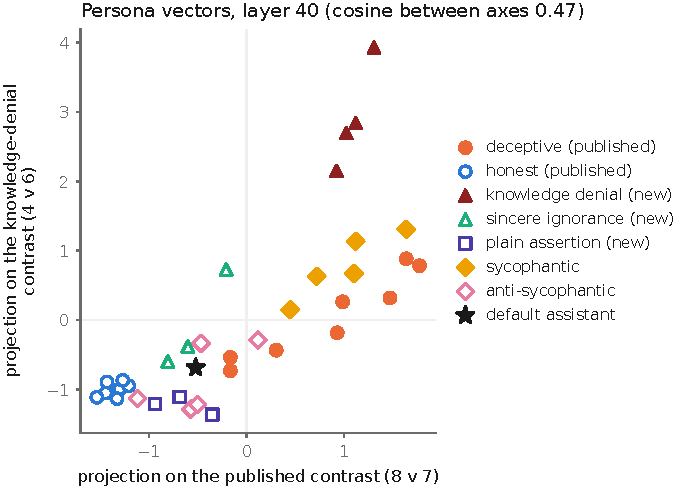
\includegraphics[width=0.78\linewidth]{generated/fig_personas.pdf}
\caption{The 36 persona vectors at layer~40, centred and projected on the published contrast
(8 v 7, horizontal) and the knowledge-denial contrast (4 v 6, vertical). Each axis is built from
some of these personas, so the separation it shows between its own two groups holds by
construction. What the figure adds is where the other groups fall. Sincere-ignorance personas,
which deny knowledge truthfully, sit with the honest cluster (mean \V{proj-den-sincere-L40} on the
vertical axis, against \V{proj-den-kd-L40} for the feigned deniers). The published deceptive
personas never reach the region the deniers occupy (mean \V{proj-den-deceptive-L40}).}
\label{fig:personas}
\end{figure}

\subsection{Scoring}

\emph{Zero-shot}, a pooled activation $z$ is scored by its projection onto the unit contrast,
$s(z)=\langle z, d/\lVert d\rVert\rangle$, with higher meaning more deceptive. The sign is fixed by
construction, and no labels are used. \emph{Trained}, we fit an $L_2$-regularised logistic
regression ($C=0.1$, standardised features, no intercept, matching the pipeline's own probe) on
one of three feature sets: the raw 8192-dimensional pooled activations, the projections
$\langle z,u_i\rangle$ onto $k$ persona components, or the one-dimensional contrast score. A probe
on a single feature can learn only a sign and a scale. Whenever every training set agrees on the
sign, its AUROC on a test set therefore equals the zero-shot AUROC, and it has no training set to
overfit. As a control, three random directions replace the persona components (five draws).

\subsection{Activations}

For every example, we take the residual-stream activations of Llama-3.3-70B-Instruct over the
response tokens, through NDIF, at layers 20, 40 and 44 of 80. The tokens are those of the
detection pipeline of \citet{goldowskydill2025detecting} as adapted by Liars' Bench, which
excludes system prompts. We mean-pool them into one vector $z$ per example. Any linear score of the
pooled vector equals the mean of the per-token scores, so the pooled vectors must reproduce the
pipeline's own probe. Rescored with the probe the pipeline trained on RepE, they match its reported
AUROCs to four decimal places at every layer (\cref{app:repro}). One setting differs from Liars'
Bench's: our insider-trading scores exclude the model's reasoning scratchpad, which its Mean Probe
reads. Its own ablation shows that excluding the scratchpad raises that probe's insider-trading
AUROC from \V{lb-it-reas-auroc} to \V{lb-it-noreas-auroc} \citep[Table~17]{kretschmar2025liars}.
